\subsection{Data Extraction in PRISM}

The analytical dataset used in this study originates from the Plastic Recovery Insights Steering Model (PRISM), a data ecosystem developed by AEPW to gather country-level plastic waste, demographic, and socioeconomic data from heterogeneous public sources.

\begin{figure}[H]
	\centering
	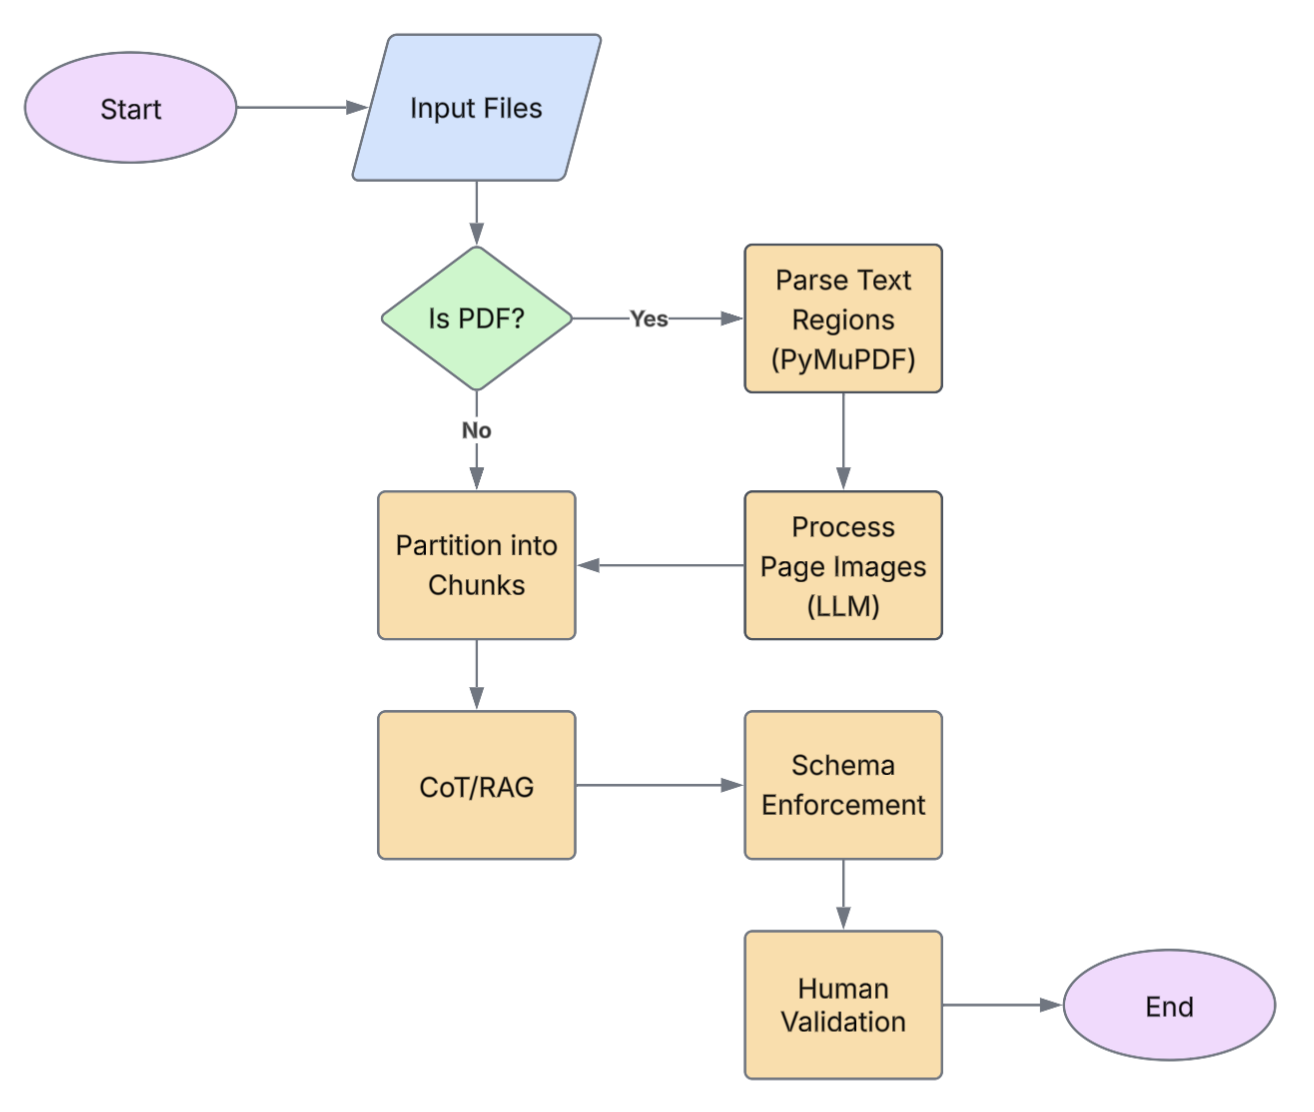
\includegraphics[width=0.8\linewidth]{figures/prism_data_extraction.png}
	\caption{
		Data extraction workflow implemented in PRISM. Input documents are first classified by format (PDF or tabular files). For PDF files, PRISM first parses text regions using PyMuPDF and processes page images using large language models. Subsequently, both PDF-derived text and tabular files are partitioned into chunks. Large language models are then used to extract data points via chain-of-thought prompting and retrieval-augmented generation. All extracted data points are subjected to schema enforcement and will undergo human validation before being used by downstream analysis.
	}
	\label{fig:prism_data_extraction}
\end{figure}

PRISM transforms heterogeneous and unstructured source files into structured analytical records through an LLM-assisted data extraction workflow (Figure~\ref{fig:prism_data_extraction}). To ensure data consistency and reliability, all extracted records are ensured to comprise location (country or region), reference year, numerical value, measurement unit, data group, and source reference. Because automated extraction can involve inevitable noise and inaccuracies, only records that have been manually reviewed and approved are admitted into the AUDA analytical database, where they are subsequently used for modeling and visualization.
